\documentclass{article}

\usepackage[nonatbib,preprint]{neurips_2024}

\usepackage[utf8]{inputenc}
\usepackage[T1]{fontenc}
\usepackage{hyperref}
\usepackage{url}
\usepackage{booktabs}
\usepackage{amsfonts}
\usepackage{nicefrac}
\usepackage{microtype}
\usepackage{xcolor}
\usepackage{amsmath}
\usepackage{graphicx}
\usepackage{tikz}
\usetikzlibrary{positioning, decorations.pathreplacing, calc}
\graphicspath{{figs/}}

\title{Benchmarking Explanation Methods on a Multi-Task Vision Transformer\\with Human Saliency Alignment}

\author{%
 Nicholas Welsh \\
  Department of Computer Science\\
  Department of Mathematics \\
  Florida Institute of Technology\\
  Melbourne, FL 32901 \\
  \texttt{nwelsh2024@my.fit.edu}
}

\begin{document}
\maketitle

\begin{abstract}
We evaluate five post-hoc explanation methods on a multi-task Vision Transformer (DeiT-Small) that jointly predicts COCO object categories and SALICON fixation maps. The setup provides a natural testbed for explainability because the model's saliency head predicts where humans look, while explanation methods produce attribution maps that highlight where the model looks. We compare gradient saliency, gradient$\,\times\,$input, integrated gradients, attention rollout, and LIME on faithfulness (deletion and insertion AUC) and human alignment (correlation with fixation ground truth), with additional stability analysis (cosine similarity under perturbations) for the two gradient-based methods. LIME achieves the best faithfulness (deletion AUC $0.409$, insertion AUC $0.881$) but the worst human alignment (CC $0.107$). Integrated gradients offers the best balance, with moderate faithfulness, highest human alignment (CC $0.248$), and highest stability. Attention rollout, designed for vanilla ViT, collapses to a single CLS-dominated patch in DeiT, producing near-zero alignment (CC $-0.003$). These results suggest that faithfulness to the model and agreement with human perception are distinct properties, and that explanation quality depends on the interaction between the method and the architecture.
\end{abstract}

\section{Introduction}

Explainable AI (XAI) methods aim to answer why a model made a particular prediction. For image classifiers, this typically means producing a spatial attribution map that highlights which input regions were most important for the output. Many such methods exist, but comparing them is difficult because there is no single ground truth for what a ``correct'' explanation looks like. Evaluation usually relies on proxy metrics such as faithfulness tests (does masking the highlighted region actually change the prediction?) or subjective human ratings.

Our setup introduces a concrete alternative. We train a Vision Transformer on COCO images paired with SALICON human fixation maps. The SALICON data tells us, for each image, where people actually look. This provides a behavioral reference for one dimension of explanation quality, namely agreement with human visual attention. A faithful explanation highlights what the \emph{model} finds important. A human-aligned explanation highlights what \emph{people} find important. These two properties need not coincide, and measuring both reveals how each explanation method balances fidelity to the model against interpretability to a human observer.

We apply five explanation methods to the trained model and evaluate each on three axes:
\begin{enumerate}
    \item \textbf{Faithfulness.} Does removing the highlighted patches actually decrease the model's confidence? (Deletion test.) Does adding them back increase it? (Insertion test.)
    \item \textbf{Stability.} Do explanations change drastically under small input perturbations (Gaussian noise, brightness shift, horizontal flip)?
    \item \textbf{Human alignment.} How well does the attribution map correlate with the SALICON fixation density?
\end{enumerate}

What is unique about visual attention is that we have a behavioral reference. In most XAI benchmarks, human alignment is either not measured or measured through subjective ratings. Here, SALICON provides continuous, per-pixel fixation density from thousands of observers, giving us a quantitative yardstick that is independent of the model.

\subsection{Contributions}
\begin{itemize}
    \item \textbf{Three-axis evaluation.} We simultaneously measure faithfulness, stability, and human alignment for five explanation methods on the same model and dataset.
    \item \textbf{Human saliency as an alignment target.} We use SALICON fixation maps as a quantitative behavioral reference for human visual attention, avoiding subjective evaluation.
    \item \textbf{Architecture-method interaction.} We document how attention rollout collapses in our 12-layer DeiT-Small, where residual-mixed matrix multiplication compounds small CLS-token asymmetries across layers.
    \item \textbf{Faithfulness vs.\ alignment trade-off.} We show that LIME, the most faithful method, has the weakest human alignment, while integrated gradients offers the best compromise.
\end{itemize}

\section{Related Work}

\paragraph{Post-hoc explanation methods.}
Gradient-based methods (Simonyan et al., 2014; Sundararajan et al., 2017) compute attribution by differentiating the output with respect to the input. Integrated gradients (Sundararajan et al., 2017) accumulates gradients along a path from a baseline to the input, satisfying axiomatic properties including completeness. LIME (Ribeiro et al., 2016) fits a local linear model by perturbing the input and observing the model's response. Attention rollout (Abnar and Zuidema, 2020) combines attention matrices across transformer layers to produce a single token-level importance map.

\paragraph{Faithfulness evaluation.}
Petsiuk et al.\ (2018) introduced the deletion and insertion metrics by progressively removing (or revealing) pixels in order of attribution importance and measuring the effect on the model's output. The area under the resulting curve quantifies how well the attribution identifies decision-relevant regions.

\paragraph{Saliency as an XAI alignment target.}
Several works have compared model attributions to human gaze data (Das et al., 2017; Bylinskii et al., 2019). These studies typically use eye-tracking data on natural images and measure correlation between model attributions and fixation density. Our work extends this line by using the same model to both predict saliency (via its saliency head) and generate explanations (via post-hoc methods), creating a controlled comparison within a single architecture.

\section{Model and Data}

\paragraph{Architecture.}
We fine-tune DeiT-Small (\texttt{deit\_small\_patch16\_224}) with two heads on the shared backbone. The classification head is a linear layer on the CLS token producing $K\!=\!20$ logits (multi-label, top 20 COCO categories). The saliency head applies a linear layer to each patch token followed by a softmax over all 196 patches, producing a $14\!\times\!14$ probability distribution. Figure~\ref{fig:architecture} illustrates the full architecture.

\begin{figure}[t]
  \centering
  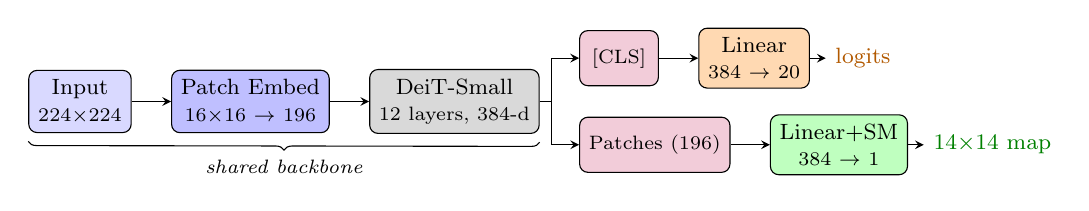
\begin{tikzpicture}[
    node distance=0.5cm,
    box/.style={draw, rounded corners=3pt, minimum height=0.7cm, align=center, font=\footnotesize},
    >=stealth
  ]
    \node[box, fill=blue!15, minimum width=1.3cm] (img)
      {Input\\\scriptsize 224$\times$224};
    \node[box, fill=blue!25, minimum width=1.4cm, right=of img] (patch)
      {Patch Embed\\\scriptsize 16$\times$16 $\to$ 196};
    \node[box, fill=gray!30, minimum width=1.7cm, right=of patch] (backbone)
      {DeiT-Small\\\scriptsize 12 layers, 384-d};
    \node[box, fill=purple!20, minimum width=1.0cm, above right=0.55cm and 0.5cm of backbone.east, anchor=west] (cls)
      {\scriptsize [CLS]};
    \node[box, fill=purple!20, minimum width=1.0cm, below right=0.55cm and 0.5cm of backbone.east, anchor=west] (ptok)
      {\scriptsize Patches (196)};
    \node[box, fill=orange!30, minimum width=1.3cm, right=of cls] (clshead)
      {Linear\\\scriptsize 384 $\to$ 20};
    \node[box, fill=green!25, minimum width=1.3cm, right=of ptok] (salhead)
      {Linear+SM\\\scriptsize 384 $\to$ 1};
    \node[right=0.2cm of clshead, font=\footnotesize, text=orange!70!black] (clsout) {logits};
    \node[right=0.2cm of salhead, font=\footnotesize, text=green!50!black] (salout) {14$\times$14 map};
    \draw[->] (img) -- (patch);
    \draw[->] (patch) -- (backbone);
    \draw[->] (backbone.east) -- ++(0.15,0) |- (cls.west);
    \draw[->] (backbone.east) -- ++(0.15,0) |- (ptok.west);
    \draw[->] (cls) -- (clshead);
    \draw[->] (ptok) -- (salhead);
    \draw[->] (clshead) -- (clsout);
    \draw[->] (salhead) -- (salout);
    \draw[decorate, decoration={brace, amplitude=3pt, mirror}]
      ([yshift=-3pt]img.south west) -- ([yshift=-3pt]backbone.south east)
      node[midway, below=3pt, font=\scriptsize\itshape] {shared backbone};
  \end{tikzpicture}
  \caption{\textbf{Multi-task ViT architecture.} A shared DeiT-Small backbone feeds a classification head on the CLS token and a saliency head on the 196 patch tokens. All XAI explanations are computed with respect to this model.}
  \label{fig:architecture}
\end{figure}

\paragraph{Training.}
The multi-task loss is $\mathcal{L} = \mathcal{L}_{\text{cls}} + \lambda\,\mathcal{L}_{\text{sal}}$ with $\lambda=1.0$. Classification uses BCEWithLogitsLoss, and saliency uses KL divergence between the predicted and target distributions. We fine-tune with AdamW (lr $10^{-4}$, weight decay $10^{-4}$) for 15 epochs with cosine annealing on 10{,}000 training images from SALICON. The best checkpoint by validation loss is used for all XAI experiments.

\paragraph{Dataset.}
SALICON provides fixation density maps for 10{,}000 train and 5{,}000 val COCO images. Ground truth saliency maps are normalized to $14\!\times\!14$ distributions (matching the ViT patch grid) for both training and XAI evaluation.

\section{Explanation Methods}

All explanations are computed on the validation set with respect to the model's most confident predicted class.

\paragraph{Gradient saliency.}
We compute $|\partial \ell / \partial x|$ where $\ell$ is the logit for the target class and $x$ is the input image. The absolute gradient is max-pooled across color channels and resized to $14\!\times\!14$.

\paragraph{Gradient $\times$ input.}
Same as gradient saliency but element-wise multiplied by the input before taking the absolute value and max-pooling across channels. This weights the gradient by input intensity, emphasizing regions where both the gradient and the signal are large.

\paragraph{Integrated gradients.}
We integrate the gradient along a straight-line path from a zero baseline to the input image using 50 interpolation steps (Sundararajan et al., 2017):
\begin{equation}
\text{IG}_i(x) = (x_i - x_i') \int_{\alpha=0}^{1} \frac{\partial F(x' + \alpha(x - x'))}{\partial x_i}\, d\alpha,
\end{equation}
where $x'$ is the zero baseline and $F$ is the target-class logit. The absolute result is max-pooled across channels and resized to $14\!\times\!14$.

\paragraph{Attention rollout.}
Following Abnar and Zuidema (2020), we multiply attention matrices across all 12 transformer layers, adding an identity matrix at each step to account for residual connections:
\begin{equation}
\hat{A}^{(l)} = 0.5\,A^{(l)} + 0.5\,I, \qquad R = \prod_{l=1}^{L}\hat{A}^{(l)}.
\end{equation}
The final row corresponding to the CLS token gives the importance of each patch. We reshape the $196$ patch values to $14\!\times\!14$.

\paragraph{LIME.}
We segment the image into a $14\!\times\!14$ grid of non-overlapping patches (matching the ViT patch grid) and train a local linear model on 300 perturbed versions of the input. Each perturbation randomly masks a subset of patches. The learned linear weights indicate the importance of each patch for the target-class probability (sigmoid output).

\section{Evaluation Metrics}

\paragraph{Faithfulness: deletion and insertion.}
For the deletion test, we progressively mask patches in decreasing order of attribution importance and record the prediction confidence at each step. The area under this curve (lower is better) measures how effectively the attribution identifies decision-critical regions. The insertion test starts from a blank image and reveals patches in decreasing importance order. Higher AUC indicates more faithful attributions.

\paragraph{Stability.}
We apply three perturbations to each input image, namely Gaussian noise ($\sigma = 0.02$ and $0.05$), horizontal flip, and brightness shift ($+0.05$). For each perturbation we re-compute the explanation and measure cosine similarity with the original. For horizontal flips, we flip the perturbed attribution map back to the original orientation before computing similarity so that the comparison is spatially aligned. Higher similarity indicates more stable explanations. We test stability on gradient saliency and integrated gradients, as these are the two gradient-based methods for which stability is most informative.

\paragraph{Human alignment.}
We compute Pearson correlation (CC) and similarity (SIM) between each attribution map and the SALICON ground-truth fixation density. Before comparison, attribution maps are resized to $14\!\times\!14$ (matching the ground-truth grid) and normalized to non-negative values. CC measures linear agreement and SIM measures histogram intersection.

\section{Results}

\paragraph{Faithfulness.}
Table~\ref{tab:xai} reports deletion and insertion AUC averaged over 100 validation samples. LIME achieves the best faithfulness by a clear margin: deletion AUC $0.409$ (lower is better) and insertion AUC $0.881$ (higher is better). This is expected because LIME is explicitly trained to approximate the model's local decision boundary by fitting a linear surrogate. Gradient-based methods cluster together, with integrated gradients slightly ahead of vanilla gradient saliency. Attention rollout is the least faithful, consistent with prior work showing that raw attention weights are noisy proxies for feature importance (Jain and Wallace, 2019).

\begin{table}[t]
\centering
\caption{XAI evaluation (100 samples, mean $\pm$ std). Del AUC: lower is better. Ins AUC: higher is better. CC: higher is better.}
\label{tab:xai}
\small
\begin{tabular}{lcccc}
\toprule
Method & Del AUC $\downarrow$ & Ins AUC $\uparrow$ & Align CC $\uparrow$ & Align SIM $\uparrow$ \\
\midrule
Gradient saliency & $0.468 \pm 0.261$ & $0.766 \pm 0.225$ & $0.161 \pm 0.238$ & $0.410 \pm 0.099$ \\
Grad $\times$ input & $0.521 \pm 0.283$ & $0.768 \pm 0.224$ & $0.171 \pm 0.241$ & $0.405 \pm 0.105$ \\
Integrated gradients & $0.479 \pm 0.261$ & $0.778 \pm 0.221$ & $\mathbf{0.248 \pm 0.251}$ & $\mathbf{0.434 \pm 0.100}$ \\
Attention rollout & $0.544 \pm 0.250$ & $0.745 \pm 0.235$ & $-0.003 \pm 0.080$ & $0.123 \pm 0.040$ \\
LIME & $\mathbf{0.409 \pm 0.306}$ & $\mathbf{0.881 \pm 0.136}$ & $0.107 \pm 0.143$ & $0.416 \pm 0.109$ \\
\bottomrule
\end{tabular}
\end{table}

\paragraph{Human alignment.}
Integrated gradients has the highest CC with human fixation data ($0.248$), followed by grad$\,\times\,$input ($0.171$) and gradient saliency ($0.161$). LIME, despite being the most faithful, has the weakest alignment among gradient-based methods (CC $0.107$). Attention rollout is near zero (CC $-0.003$), indicating no systematic relationship with human gaze.

This dissociation between faithfulness and alignment is the central finding. LIME is faithful because it directly models what the classifier relies on. But what the classifier relies on need not be what humans look at. The model may use texture, context, or background cues that are invisible to naive human inspection. Integrated gradients strikes a middle ground: it aggregates information along the full interpolation path, which tends to produce smoother and more spatially coherent maps that happen to overlap with fixation density.

\paragraph{Attention rollout collapse in our setup.}
Attention rollout was designed for shallow transformers where attention is relatively distributed across tokens. In our 12-layer DeiT-Small, multiplying attention matrices across all layers with residual mixing ($0.5A + 0.5I$ at each step) causes small asymmetries in attention toward the CLS token to compound with depth. The resulting rollout map concentrates almost all weight on one or two patches regardless of image content. Figure~\ref{fig:comparison} shows this visually: attention rollout produces a near-black map with one bright cell. We believe this reflects a numerical limitation of deep attention rollout (Abnar and Zuidema, 2020), where repeated matrix products converge to a degenerate distribution, though we have not tested whether the same collapse occurs in other architectures or at different depths.

\begin{figure}[t]
  \centering
  
\includegraphics[width=\linewidth]{report_comparison_323.png}
  \caption{\textbf{Explanation comparison} on a validation image (dog + fire hydrant). Gradient-based methods highlight the dog. LIME highlights a broader region. Attention rollout collapses to a single patch. The contrast illustrates how different methods capture different aspects of the model's reasoning.}
  \label{fig:comparison}
\end{figure}

\paragraph{Stability.}
Table~\ref{tab:stability} shows stability results for gradient saliency and integrated gradients under four perturbation types. Integrated gradients is more stable across all perturbations, particularly under horizontal flip (cosine similarity $0.820$ vs $0.768$). The path integration in IG acts as a smoothing operation that reduces sensitivity to small input changes. Both methods are highly stable under brightness shifts, suggesting that DeiT features are largely invariant to uniform intensity changes.

\begin{table}[t]
\centering
\caption{Stability: cosine similarity between original and perturbed explanations (higher = more stable).}
\label{tab:stability}
\begin{tabular}{lcccc}
\toprule
Method & Noise $\sigma\!=\!0.02$ & Noise $\sigma\!=\!0.05$ & H-flip & Brightness \\
\midrule
Gradient saliency & 0.963 & 0.918 & 0.768 & 0.988 \\
Integrated gradients & 0.990 & 0.969 & 0.820 & 0.999 \\
\bottomrule
\end{tabular}
\end{table}

\paragraph{Qualitative examples.}
Figure~\ref{fig:comparison} shows a representative comparison. On this image of a dog next to a fire hydrant, gradient saliency and integrated gradients both concentrate on the dog (the predicted class). Integrated gradients produces a tighter, more focused map. LIME highlights a broader region including the ground near the dog. Attention rollout shows a single bright patch unrelated to either object. The SALICON fixation map (not shown) concentrates on the dog and hydrant, most closely matching the integrated gradients map.

\begin{figure}[t]
  \centering
  
\includegraphics[width=\linewidth]{report_comparison_305.png}
  \caption{\textbf{Explanation comparison} on a second validation image (tennis player). All gradient-based methods roughly agree on the player's location. LIME assigns high importance to the court surface, suggesting the model uses background context for its prediction.}
  \label{fig:comparison_2}
\end{figure}

\section{Discussion}

\paragraph{Faithfulness $\neq$ human alignment.}
The most important takeaway is that these two properties are distinct, even inversely related in some cases. LIME achieves the best faithfulness because it is explicitly optimized to approximate the model's local behavior. But the model's decision-relevant features may not correspond to where humans look. This distinction matters in practice: if the goal is to debug or audit a model, faithfulness is the right metric. If the goal is to produce explanations that a human can verify against their own perception, alignment matters more.

\paragraph{Integrated gradients as a practical default.}
Among the five methods tested, integrated gradients offers the best overall profile with moderate faithfulness, highest human alignment, and highest stability. Its axiomatic guarantees (completeness, sensitivity) provide theoretical grounding, and the path integration produces smooth, interpretable maps. The main drawback is computational cost (50 forward passes per sample), which is acceptable for offline analysis.

\paragraph{Limitations.}
Our evaluation uses a single model (DeiT-Small) and dataset (SALICON/COCO), and the validation set serves for both checkpoint selection and final evaluation since SALICON does not provide a public test split with ground truth. The attention rollout collapse is consistent with numerical degeneration from deep matrix multiplication with residual mixing, and its severity may vary across architectures and depths. The human alignment comparison is limited by the resolution mismatch: attributions and fixation maps are both downsampled to $14\!\times\!14$, which may obscure fine-grained spatial differences. We evaluate on 100 samples, which provides stable means but wide standard deviations (see Table~\ref{tab:xai}), reflecting genuine per-image variability.

\section{Conclusion}

We evaluated five explanation methods on a multi-task Vision Transformer using SALICON fixation maps as a behavioral reference for human visual attention. The results point to a tension between these properties. LIME is the most faithful to the model but the least aligned with human gaze. Integrated gradients offers the best compromise across all three evaluation axes. Attention rollout, while conceptually appealing, failed in our DeiT-Small setup, where residual-mixed matrix products compound CLS-token asymmetry across 12 layers. These findings suggest that explanation method selection should be guided by the intended use case (model debugging vs.\ human communication) and the specific architecture.

\paragraph{Reproducibility.}
All experiments use seed 42. Code is available at \href{https://github.com/nickvpn/vit-ml-xai-project}{github.com/nickvpn/vit-ml-xai-project}.

\begin{thebibliography}{12}

\bibitem{simonyan2014}
Simonyan, K., Vedaldi, A., and Zisserman, A.\ (2014).
Deep Inside Convolutional Networks: Visualising Image Classification Models and Saliency Maps.
\textit{ICLR Workshop}.

\bibitem{sundararajan2017}
Sundararajan, M., Taly, A., and Yan, Q.\ (2017).
Axiomatic Attribution for Deep Networks.
\textit{ICML}.

\bibitem{ribeiro2016}
Ribeiro, M.~T., Singh, S., and Guestrin, C.\ (2016).
``Why Should I Trust You?'': Explaining the Predictions of Any Classifier.
\textit{KDD}.

\bibitem{abnar2020}
Abnar, S.\ and Zuidema, W.\ (2020).
Quantifying Attention Flow in Transformers.
\textit{ACL}.

\bibitem{petsiuk2018}
Petsiuk, V., Das, A., and Saenko, K.\ (2018).
RISE: Randomized Input Sampling for Explanation of Black-box Models.
\textit{BMVC}.

\bibitem{jain2019}
Jain, S.\ and Wallace, B.~C.\ (2019).
Attention is not Explanation.
\textit{NAACL}.

\bibitem{das2017}
Das, A., Agrawal, H., Zitnick, C.~L., Parikh, D., and Batra, D.\ (2017).
Human Attention in Visual Question Answering: Do Humans and Deep Networks Look at the Same Regions?
\textit{CVIU}, 163, 90--100.

\bibitem{bylinskii2019}
Bylinskii, Z., Judd, T., Oliva, A., Torralba, A., and Durand, F.\ (2019).
What Do Different Evaluation Metrics Tell Us About Saliency Models?
\textit{IEEE TPAMI}, 41(3), 740--757.

\bibitem{dosovitskiy2021}
Dosovitskiy, A., Beyer, L., Kolesnikov, A., et al.\ (2021).
An Image is Worth 16x16 Words: Transformers for Image Recognition at Scale.
\textit{ICLR}.

\bibitem{touvron2021}
Touvron, H., Cord, M., Douze, M., et al.\ (2021).
Training Data-Efficient Image Transformers \& Distillation through Attention.
\textit{ICML}.

\bibitem{jiang2015}
Jiang, M., Huang, S., Duan, J., and Zhao, Q.\ (2015).
SALICON: Saliency in Context.
\textit{CVPR}.

\end{thebibliography}

\end{document}
